\documentclass[11pt]{article}
\usepackage{tikz}
\def\checkmark{\tikz\fill[scale=0.4](0,.35) -- (.25,0) -- (1,.7) -- (.25,.15) -- cycle;} 
\usepackage{proj} 	% pull in style header
\usepackage{array}
\usepackage{sectsty}

\lhead{ECE540: SoC Design with FPGA's}

%TODO: Put in coverpage from hw1, with tunnel vision image.  

%----------------------------------------------------------------------------------------
%	TITLE SECTION
%----------------------------------------------------------------------------------------


\newcommand{\horrule}[1]{\rule{\linewidth}{#1}} % Create horizontal rule command with 1 argument of height

\title{	
\normalfont \normalsize 
\textsc{\LARGE Portland State University}\\[1.5cm] % Name of your university/college
\textsc{\Large SoC Design With FPGAs}\\[0.5cm] % Major heading such as course name
\textsc{\large ECE540}\\[0.5cm] % Minor heading such as course title
%\textsc{Portland State University} \\ [25pt] % Your university, school and/or department name(s)
\horrule{1.2pt} \\[0.4cm] % Thin top horizontal rule
\huge Tunnel Vision \\ % The assignment title
\horrule{1.2pt} \\[0.5cm] % Thick bottom horizontal rule
}

%----------------------------------------------------------------------------------------
%	AUTHOR SECTION
%----------------------------------------------------------------------------------------
\begin{document}
\author{Erik Rhodes \and Bhavana Dhulipala \and Rohan Deshpande \and Nikhil Patil} % Your name
\maketitle % Print the title
\thispagestyle{empty}
\cfoot{\textit{Page \thepage { of} \pageref{LastPage}}}
\lhead{ECE540: SoC Design}
\chead{Tunnel Vision}
\rhead{Final Project}


\vspace{1in}
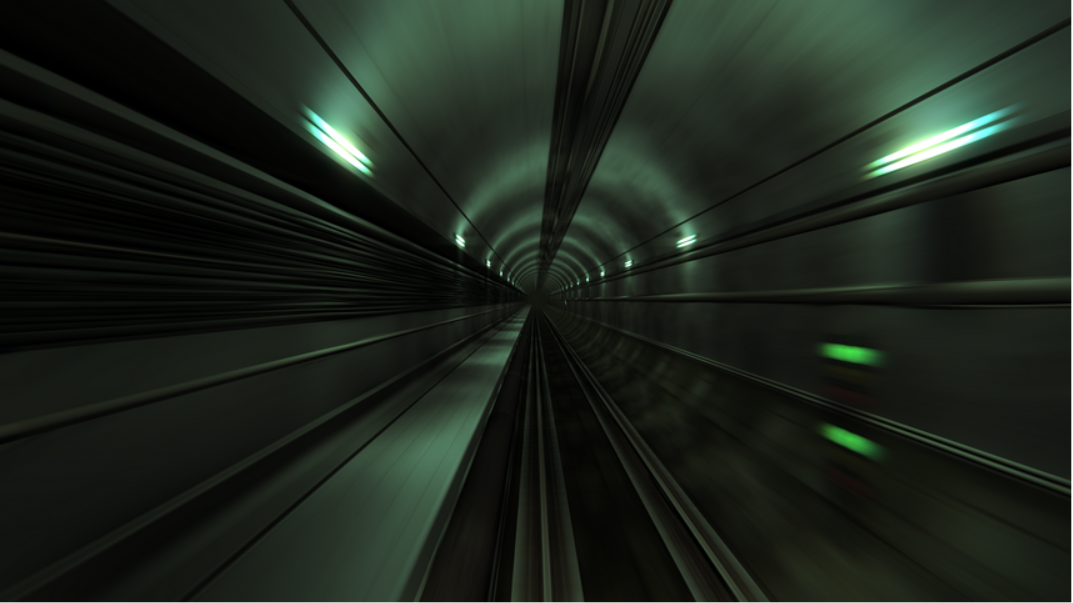
\includegraphics[height=0.5\textwidth]{Images/tunnel_graphic.png}\\

%
%\title{\textbf{ECE540: Final Project}\\Tunnel Vision}
%\author{Erik Rhodes and Bhavana Dhulipala}
%\date{February 4, 2014}

%\begin{document}
%	\maketitle{}
%	\thispagestyle{empty}
%	\newpage 
%	
%%		\thispagestyle{empty} % back of cover page is blank
%%		\vspace*{0.5\paperheight}
%%		\begin{center}
%%		{\it This page intentionally left blank}
%%		\end{center}
%%		\newpage
%		\begin{center}
%			\tableofcontents
%			\newpage
%	\end{center}


%Start of Document

% PUT IN CODE?
% put in design specs - Pictures: Top module, Hardware specifications?

\section{Introduction} 

What is tunnel vision, in general how does it play?
%	\newpage	
	\begin{figure}[t!]\centering
	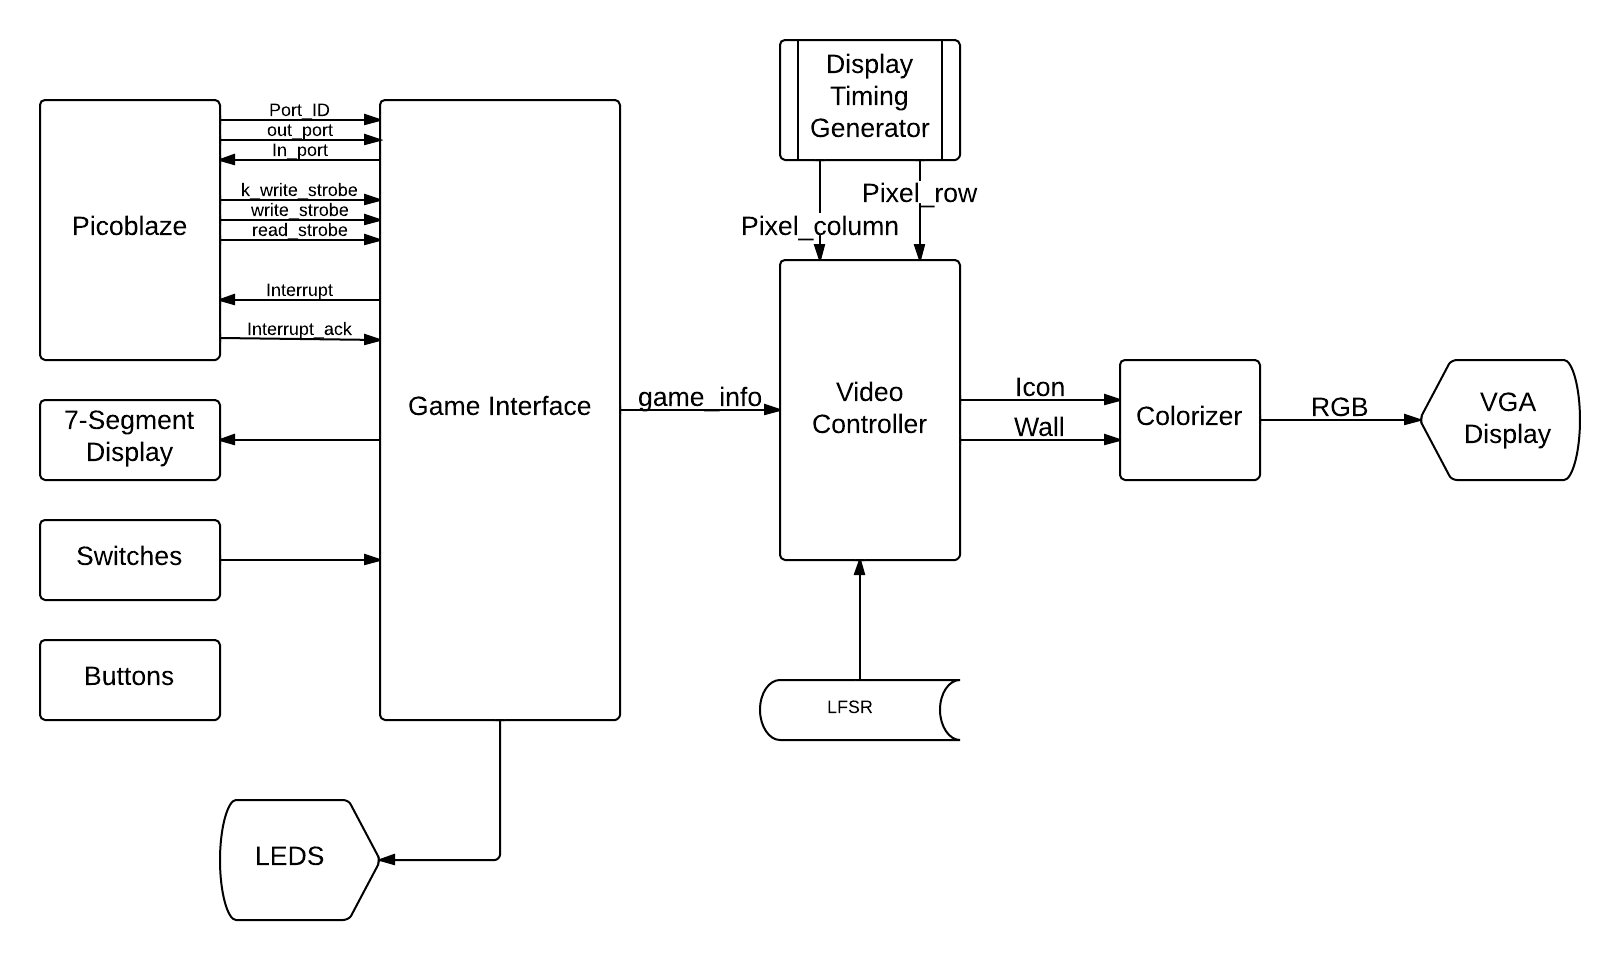
\includegraphics[height=0.8\textwidth]{Images/gameplay_diagram.png}
	\caption{Gameplay Block Diagram}
		\label{block_diagram}
	\end{figure}	

%\section{Design Specifications}
		
\section{Software Implementation}
		
		Picoblaze assembly code was used to implement the algorithm controlling the 
		vehicle's movement.
		Game logic, controls, score, levels, etc...
		
		\begin{figure}[t!]\centering
		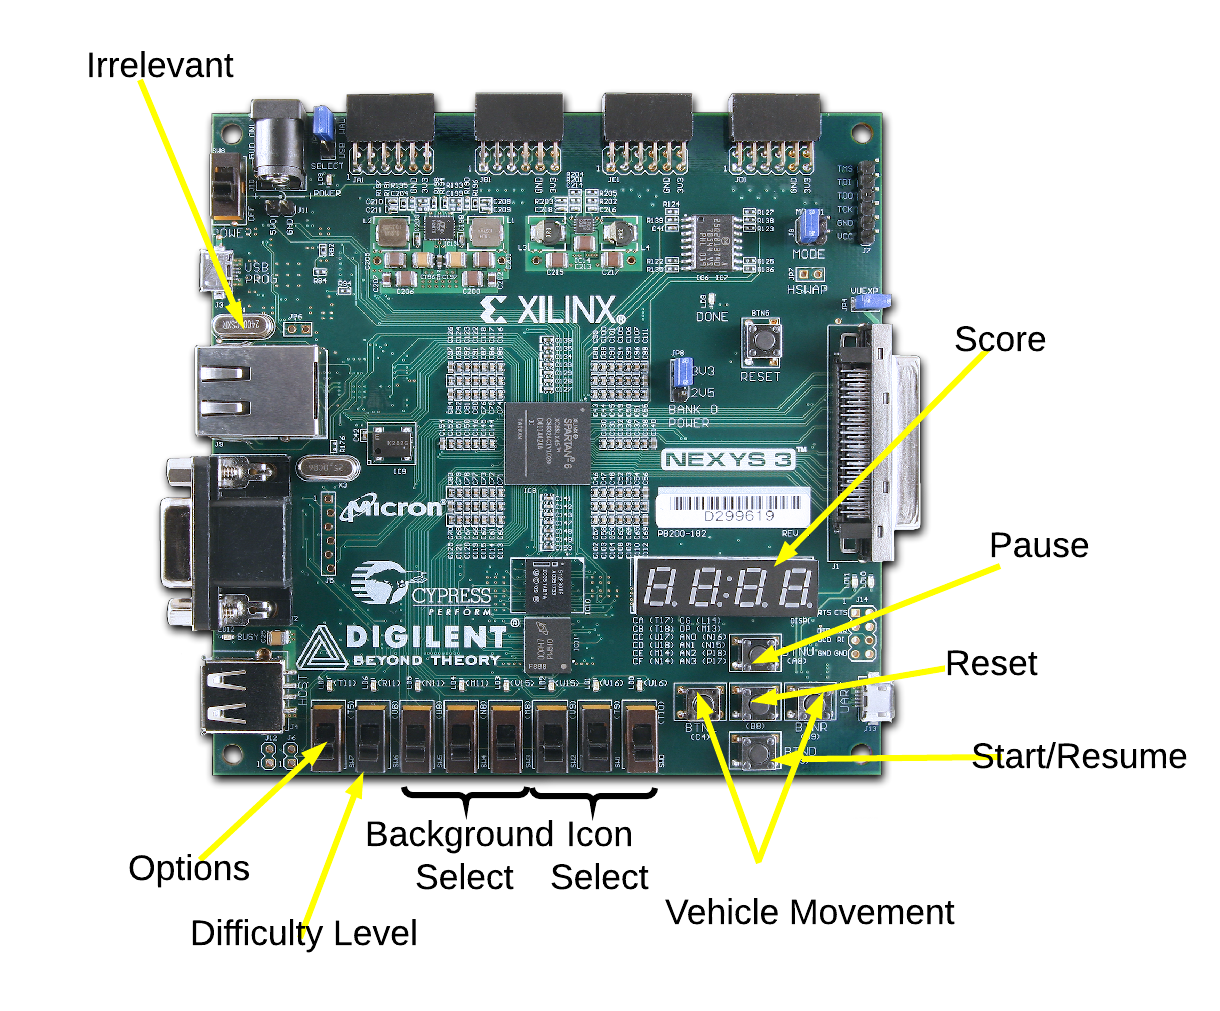
\includegraphics[height=0.8\textwidth]{Images/controls_mockup.png}
		\caption{Bot Control Flowchart}
			\label{controls}
		\end{figure}	
	 	



		
		%	\subsection{Forward}
			
Insert various code here

\begin{lstlisting}[caption=Sequence used manage orientation counter , label=loc_check]		
		LOAD	s0, 	LocX
		FETCH	s1,		SP_OLD_LOCX			;see if our current location is different
		COMPARE	s1,		s0						;if it is, we must be moving forward on a black line
		CALL	NZ,		clear_counter		;we can clear the orientation counter at this point 	
 \end{lstlisting}

			
\section{Video Controller Implementation}
	The video controller module was designed...
	The icon, wall, and different backgrounds implementation
	
%	\begin{figure}[t!]\centering
%	\includegraphics[height=0.5\textwidth]{video_controller.png}
%	\caption{Video Controller Overview}
%		\label{controller}
%	\end{figure}
		
		\subsection{Colorizer}
		

%		\begin{figure}
%		\centering
%		\begin{minipage}{.5\textwidth}
%			\centering
%		  	\includegraphics[width=.6\textwidth]{icon.png}
%		  		\caption{Icon Module}			
%			\label{icon}
%		\end{minipage}%
%		\begin{minipage}{.5\textwidth}
%		  	\centering
%			\includegraphics[width=.6\textwidth]{colorizer.png}
%			\caption{Colorizer Module}
%		  		\label{colorizer}
%		\end{minipage}
%		\end{figure}
%
%		\begin{figure}[t!]\centering
%		\includegraphics[height=0.3\textwidth]{colorizer_table.png}
%		\caption{Colorizer Table}
%			\label{colorizer_table}
%		\end{figure}
				

				
		\subsection{Icon}
		


%		\begin{figure}
%		\centering
%		\begin{minipage}{.5\textwidth}
%		  \centering
%		  \includegraphics[width=.6\textwidth]{icon_bitmap_3.png}
%		  \caption{Regular Image Translation}
%		  \label{reg_translation}
%		\end{minipage}%
%		\begin{minipage}{.5\textwidth}
%		  \centering
%		  \includegraphics[width=.6\textwidth]{icon_bitmap_4.png}
%		  \caption{Tilted Image Translation}
%		  \label{tilted_translation}
%		\end{minipage}
%		\end{figure}
					
		\begin{figure}[t!]\centering
		  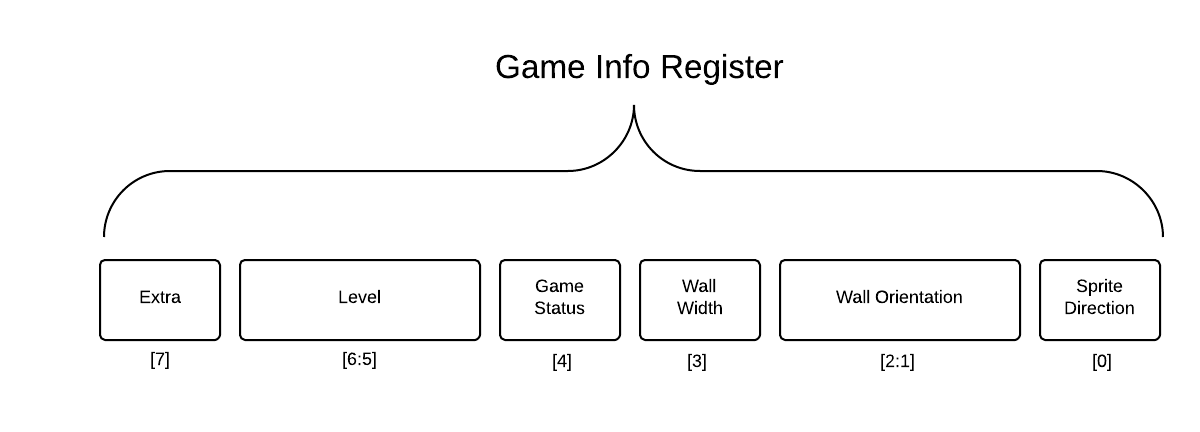
\includegraphics[width=.8\textwidth]{Images/game_info_bits.png}
		  \caption{Allocation of bits in game\_info register}
		  \label{game_info_bits}
		\end{figure}
		
		
		% first column
%\begin{minipage}[l]{0.5\textwidth}
%		\begin{itemize}

		
%\end{itemize}
%\end{minipage}\begin{minipage}[r]{0.5\textwidth}
%	\hspace{20pt}\includegraphics[width=0.9\textwidth]{../resources/mockup.png}
	
%	\hspace{50pt}Figure 1: Mockup of game screen


\section{Conclusion}
Length of time, github, results, etc.

	\subsection{Challenges}
		
		\begin{itemize}				
	
		\item Basically issues 
		
		\item problems we had
				
		\end{itemize}
	\subsection{Time Invested}

	
	
	%table "Division of Tasks" 
	\begin {table}[H]
	\begin {center} 

	\vspace{15pt}
	
	\begin{tabular}{||l|c|c||}\hline	
						& Erik Rhodes 	& Bhavana Dhulipala \\\hline
	bot\_ctrl.psm 		&	\checkmark 	&					\\\hline
	nexys\_bot\_if.v	&				&	\checkmark		\\\hline
	nexys3fpga.v		&	\checkmark	&	\checkmark		\\\hline	
	colorizer.v			&				&	\checkmark		\\\hline
	icon.v				&				&	\checkmark		\\\hline

	
	\end{tabular}
		\caption {Division of Tasks} \label{Division of Tasks}
	\end{center}
	\end{table}
	\subsection{Future Work}
	While our project completed all requirements and executed perfectly, there is still room for improvement. Future modifications would include:
	
	\begin{itemize}
	\item \textbf{Multiplayer Mode:} 
	\end{itemize}
\end{document}